\chapter{Design}
%Overall design goals:
%The converter is open to extension and modification
%The code should be easy to extend and modify
% - Requires code that is easy to understand
Now that both data formats have been analyzed and conversion schemes have been proposed, a system can be designed to support this conversion. This section will explain the system architecture and its design process. Initially in section 5.1, a framework system is designed that deals with the practical requirements and limitations of the conversion and acts as a container for the conversion modules. Such requirements and limitations include considering how to exchange data with the converter. Section 5.2 gives an overview of the design goals that are rooted in aesthetics and propose design approaches how to achieve them. Such design goal include ease-of-use (simplicity) and maintainability (code management). Section 5.3 presents how the system's component structure divides the conversion process into multiple steps. Section 5.4 shows how a certain independence between those components can be achieved. Finally, the base structure of the converter components is explained in section 5.5.


%\comg{We now proceed to the design of the system to support the conversion between the two data formats.} This section will explain the system architecture and its design process, starting by showing how the base system is rooted in its requirements. Then, the level of detail will increase step by step, by looking at the design of various converter components. This way, the underlying design ideas will be revealed before diving into the details of the system.

%\commentGeorgios{This section includes a high level of technicality and it is difficult for the reader to understand. Be more specific and explain in a great level of detail what is the goal of each subsection. For example: In 5.1, we recast the requirements of the system to be build after considering our initial proposal and the research conducted in the analysis section. In subsection 5.2, we specify the development goals and base our design approach to some good software engineering practices. Section 5.3 does this with 1-2 sentences. Section 5.4 does this with 1-2 sentences. Section 5.5 does this. Moreover, about 5.3,5.4,5.5 take care of the order of presenting these sections. I understood more or less what you did, but your goal is to help, guide, and facilitate the reader to understand what you did..}

\section{System requirements and limitations}
The most basic requirement of the converter, is that it must be able to convert SBML-qual to ERODE-format and vice versa. To do so, the converter must be capable of basic input/output of files (file-I/O), as a standalone program. Once the converter has read its input file, it must be able to extract the required data from the file. For SBML this can be done using the JSBML-library, a Java-API to read and write SBML files. In case of the ERODE format, the ERODE-library is capable of file-I/O, but only to the extent of writing. This means, that the standalone converter can only generate ERODE-files from an SBML input, but not vice versa. The compiler used to interpret the ERODE format (.ode) is also not publicly available, which is why there are no means to parse ERODE-files directly in the converter.
However, the converter must still be able to converter ERODE's data representation into SBML format, since it still could be used inside ERODE to export to SBML. To enable the converter to convert from ERODE to SBML, the reading and writing of files, simply needs to be separated from the conversion process itself. In other words, by converting between the data representations used by ERODE and JSBML. This will essentially outsource all file-I/O to the JSBML and ERODE plugins, and turn the converter into a bridge between the two formats. 

\begin{figure}[H]
    \centering
    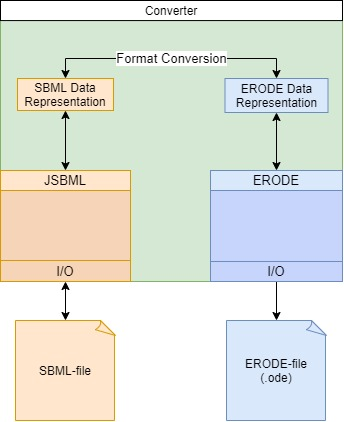
\includegraphics[scale=0.45]{Sections/Images/ConverterSystem.jpg}
    \caption{An overview of the conversion system}
    \label{fig:converter_overview}
\end{figure}

As shown in figure \ref{fig:converter_overview}, the converter will be given an SBML file to convert. The converter will then take the data representation of the file and convert it to the other data representation, which then is written to a file. When integrated into ERODE, the converter will be given directly from the host program, and generate an SBML file representing the given model as output.

\section{Development goals and design approach}
Now that the basic system has been designed based on its requirements, it is time to think about how such a system can be realized in practice. That means deciding:
\begin{itemize}
    \item How file-I/O should work in this system.
    \item How the data conversion component should be designed and structured.
    \item How modifiable the system should be.
\end{itemize}
For the standalone converter, the first question is relatively simple to answer. Since both the JSBML- and the ERODE-plugin are contained within the converter, the converter itself must have a file-I/O interface of its own. This interface must be able to take in an SBML-file as an input and return a new ERODE-file as output.

The answers to the second and third question are intertwined, as the design of the conversion component will define how dependent the converter will be on the current state of both formats. Since the ERODE-tool still is in development and therefore subject to change, the converter should have a design that easily can be adapted to support changes in both formats. This requires the converter to be designed in a way that is both easy to maintain, whilst being highly modifiable.

This can be achieved using the SOLID-principle, which consists of the basic rules to create highly maintainable and extendable applications using object oriented programming. The principle itself is a collection of five principles:
\begin{itemize}
    \item \textbf{S}: The \textit{single responsibility principle} states that software components should be kept small and dedicated towards a single specific task. This will keep code segments shorter, as well as easier to understand and change.
    \item \textbf{O}: The \textit{open-closed principle} states that existing software components should be open to extension but closed for modification. This means, that any existing functionality of a component should remain unchanged, as any changes may impact the whole system. In this the case of the converter, it may not always be possible to ensure that the design always follows this principle. Since the conversion formats still are being developed, it may become necessary modify existing functionality of the converter to adapt to changes in both formats.
    \item \textbf{L}: The \textit{Liskov substitution principle} states that components that are derived from other components should be able to replace the component they were derived from without causing unexpected results.
    \item \textbf{I}: The \textit{interface segregation principle} state that interfaces should never force components to support interface-methods that should not be supported by the component. Instead such an interface should be broken down into smaller ones that can be implemented selectively.
    \item \textbf{D}: The \textit{dependency inversion principle} states that components should depend on interfaces instead of direct dependencies. This increases their independence and allows components that implement the same interface to be used interchangeably.
\end{itemize}

It should be remarked that these definitions are based on the SOLID definitions given in \href{https://learning.oreilly.com/library/view/apex-design-patterns/9781782173656/ch01s10.html#ch01lvl2sec8}{Apex Design Patterns} by \emph{Jitendra Zaa} and \emph{Anshul Verma}

\section{Converter layering}
The analysis of SBML-qual in section 4.2 revealed the complex multilayered structure of the SBML-format. Due to the complexity, the conversion to and from SBML is therefore quite an extensive task. However, this task can be broken down in to smaller sub-tasks by separating the layers and converting them in different converter components. This layer separation also reduces the responsibilities of each converter component, since each component only operates on a single layer. This enforces the \emph{single responsibility principle}.

%During the analysis of SBML-qual it quickly became visible that SBML-qual models are fairly complex structures consisting of many layers. By creating a separate converter component for each of these layers, the conversion process can be broken down into multiple smaller steps. This makes each component responsible for a single layer of the SBML-qual structure in the conversion process, enforcing the \emph{single responsibility principle}.

%\comg{A preliminary analysis of SBML-qual revealed the multilayered complex structure of the SBML-format. We initially broke down the conversion process into multiple steps. Each step consists of a separated component converter dedicated to each layer. In other words, each component is responsible for a single layer of the SBML-qual structure in the conversion process satisfying the \emph{single responsibility principle}.}
\begin{figure}[H]
    \centering
    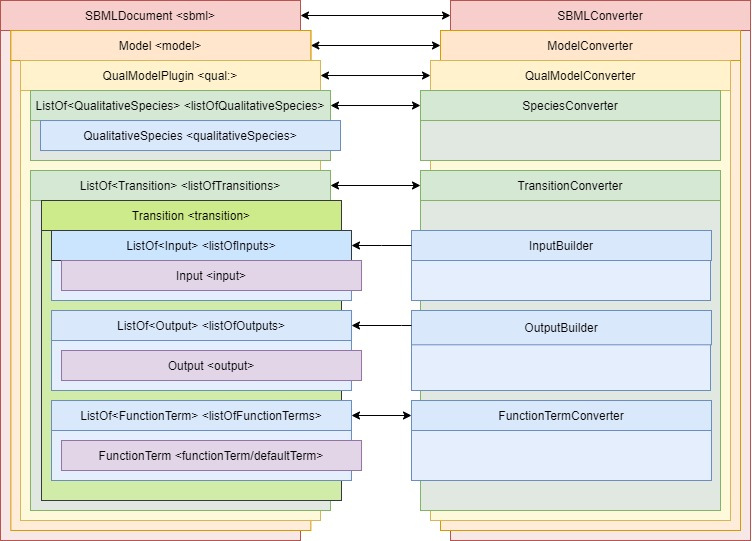
\includegraphics[scale=0.45]{Sections/Images/ConverterLayering.jpg}
    \caption{Mapping of SBML-qual layer to corresponding converter component}
    \label{fig:converterLayering}
\end{figure}
Figure \ref{fig:converterLayering} shows the SBML-qual structure to the left and the converter's component structure to the right. Components that are enclosed by an outer component, are contained within their outer component. The coloring indicates which components are located within the same layer. The arrows are used to indicate which of the converter's components are responsible for the conversion of specific layer in the SBML-qual structure. As an example, the \emph{ModelConverter} is responsible for the conversion of the \emph{Model}-layer in SBML-qual.

The arrows also indicate, which conversion the various converter components are responsible for. Arrows pointing at the converter indicate that the component is responsible for the conversion of SBML to ERODE format. Arrows pointing at the SBML-qual structure indicate the opposite, the conversion from ERODE to SBML-qual.

Components in the SBML-qual structure that are not connected to a converter component via an arrow, are converted as a part of their enclosing layer. This also counts for SBML-layers that only are pointed at by a converter component. For example, each \emph{input} (<input>) is converted as a part of the list of inputs (<listOfInputs>) it is contained by. The list of inputs is generated by the \emph{InputBuilder}, when converting to SBML-format, but it is converted as a part of each transition, when converting to ERODE's format.

The reason, why some of these layers are converted along with their outer layers is that the outer layer for one or both conversion directions, simply does not contain enough data of its own. For example, list are used to contain multiple item of the same type, but apart from these items they contain no relevant data of their own.

%Figure \ref{fig:converterLayering} shows the layer separation achieved by mimicking the SBML-qual structure using the converter components.\comg{explain the figure better. The left part of the figure displays this. the right part of the figure displays this. The arrows indicate that...} The arrows indicate, which component is responsible for which SBML-qual layer and \comg{the nature of the responsibility} what kind of responsibility it is. \comg{ERODE does not require data from each layer of the SBML-structure, so the converter allows unnecessary layers to be omitted in the conversion process. Hence, we use two-way connections to } Two-way connections indicate that the responsible converter component is responsible for both conversion directions (SBML to ERODE and vice versa), whereas the arrows pointing at the SBML-structure indicate that these components only are required during the conversion from ERODE to SBML. Instance layers, such as the \texttt{QualitativeSpecies}- or \texttt{Input}-layer are converted along with their enclosing list layer, as they only have the logistical purpose of containing multiple items of the same type.

Now that the overall converter structure has been designed, it is important to consider how the converter components interact with each other during the conversion. This requires a step by step analysis of the conversion process.
\begin{figure}[H]
    \centering
    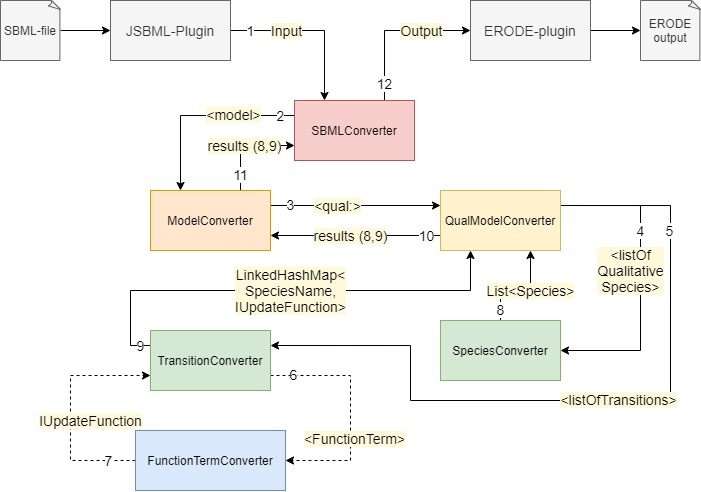
\includegraphics[scale=0.45]{Sections/Images/SBMLConversion.jpg}
    \caption{SBML to ERODE conversion process}
    \label{fig:SBMLConversion}
\end{figure}
As shown in the steps 1-3 of figure \ref{fig:SBMLConversion}, the outer converter components simply remove the outer-most layer of the SBML-qual input they are given and pass on the remaining data to the next component. This is the only requirement for the first two components since the outer SBML-layers contain only meta-data about the model, which is not required by ERODE. Thereafter, the \texttt{QualModelConverter} splits the data representation as shown in steps 4 and 5, since species and transitions are independent structures that do not require data about the other during their conversion. Because species do not contain sub-layers, the \texttt{SpeciesConverter} can convert each species and return a list of all species in ERODE format to the \emph{QualModel converter} (steps 4 and 8).

To convert transition and additional conversion step, the conversion of \emph{function terms}, is required. This is handled by the \emph{FunctionTermConverter} in steps 6 and 7, which receives a \emph{function term} from the \emph{TransitionConverter} and returns the function expression within as an \emph{IUpdateFunction}. The \emph{IUpdateFunction} is the corresponding structure in ERODE. The steps 6 and 7 are highlighted using dotted arrows, as they have to be repeated for each single transition. This means that these steps will run on a loop until all transitions have been converted.
In steps 8 and 9, the species and transitions are then returned in ERODE format, which then are routed back to the conversion entry/exit point in the \texttt{SBMLConverter}. As a final step, the \texttt{SBMLConverter} will then package the converted ERODE structures into an ERODE model, which is passed on to the ERODE plugin to generate the file.

Apart from a few minor details, the reverse conversion, from ERODE to SBML, largely corresponds to the execution process in figure \ref{fig:SBMLConversion}, but in reverse. The main differences are the the \emph{input} and \emph{output} builders from figure \ref{fig:converterLayering} need to be included to generate SBML transitions and that the ERODE model is supplied by the ERODE host program instead of a file.

\section{Component separation}
When looking back at, how each of these converter components exchange data, it quickly becomes visible that all components request data from components in a lower layer (sub-components), whereas they always respond to a component in a higher layer (parent). Since that is the case, all components can be separated by introducing interfaces that define the contract for their communication. This enforces the \emph{dependency inversion principle} and increases the maintainability of the converter even further, by design.
\begin{figure}[H]
    \centering
    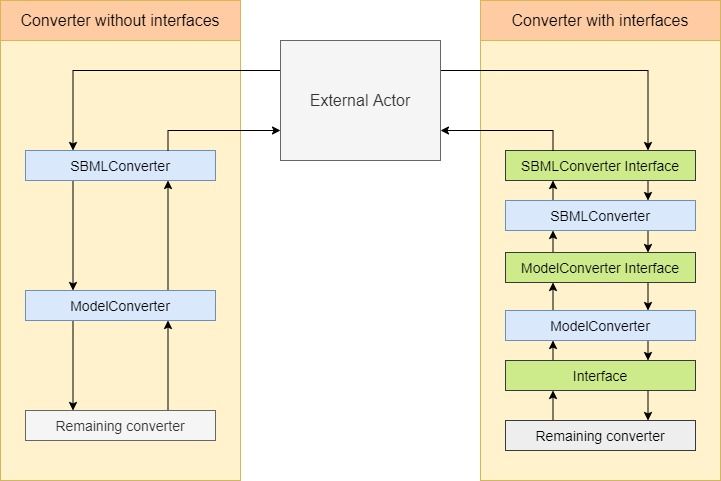
\includegraphics[scale=0.45]{Sections/Images/Interfacing.jpg}
    \caption{Converter structure with and without interface}
    \label{fig:interfacing}
\end{figure}
When comparing the two converters shown in figure \ref{fig:interfacing} it can be seen that the converter without interfaces consists of components that depend on each other directly, this means that there is one specific type of component that is required to ensure the conversion can succeed. 
The other converter on the other hand relies on interfaces, which act as contracts of interaction. Since it relies on interfaces instead of a direct dependency, components are implemented completely independent of each other. Implementations are hidden by the interface allowing components that implement the same interface to be used interchangeably.

\section{Component structure}
Another way of increasing maintainability by design, is to divide each converter component into sub-components. Since each component currently is responsible for both conversion directions, they can be divided into separate pieces internally. From the outside there still is only one component to interact with, but internally the two ways of conversion are handled by different sub-components.
To facilitate this, each component would require some kind of manager that can identify, which conversion process is required and initializes it accordingly.
\begin{figure}[H]
    \centering
    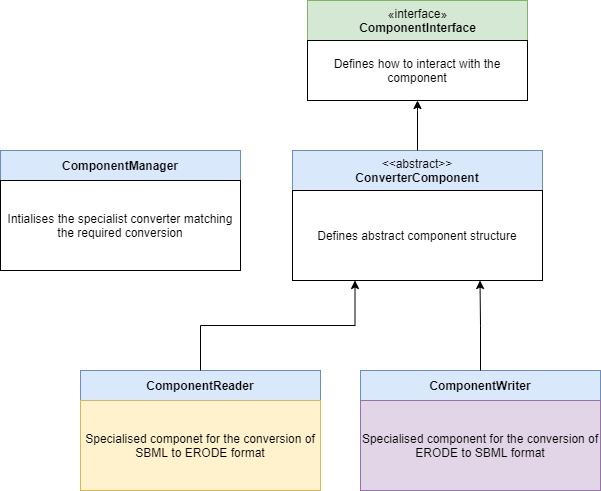
\includegraphics[scale=0.45]{Sections/Images/ComponentStructure.jpg}
    \caption{General component structure}
    \label{fig:component}
\end{figure}
As it can be seen in figure \ref{fig:component}, each component is controlled by a manager that initializes the required conversion unit. The possible interactions with the conversion unit from outside the component is defined by the \emph{ComponentInterface}. The interface is implemented by the \emph{ConverterComponent}, an abstract class defining the general converter unit's object-structure. The \emph{ConverterComponent} is extended by the \emph{reader}- and \emph{writer}-units, which define the specialized conversions of both formats. 

All conversion unit \emph{readers}, take care of \emph{reading SBML}, converting it to ERODE format, whereas \emph{writers} take ERODE format as input, \emph{writing} it to SBML. This naming convention is used to indicate the conversion direction for each of these components without needing to use either SBML or ERODE as a part of the class' name.
It should be added that this general structure may vary slightly from component to component, as some components may require additional functionality, which according to the SOLID-principle would need to be added as separate entities.
%As shown in figure \ref{fig:SBMLConversion} each converter will consume the outer most SBML-layer and pass its sub-components on to the next converter. The SBML-layer passed on is indicated by the highlighted SBML-tag on each link in the figure, e.g the \texttt{<model>} on link $2$. The converters at the lowest level will the convert their SBML-data to ERODE format first, pass the converted data back to their parent-converter. Keep in mind, that steps $6$ and $7$ might occur multiple times on a loop, as most Boolean networks consist of multiple transitions. Once, the low-level conversion is completed, the parent converters will then pack the returned ERODE-data into the required ERODE-structures. Since the packing of ERODE structures requires less layers than SBML, the remaining top-level converters will simply route the data out of the conversion module, so that it can be printed to the output-file by the ERODE-plugin. These routing steps are indicated by the \texttt{results} links.
%When considering the various steps of the conversion process, it is clear that the system in its current form is well suited to convert SBML-qual to ERODE format. On the other hand, when it comes to the reverse case, where the ERODE-format is converted to SBML-qual, the system design becomes flawed. In its current state (see figure \ref{fig:converterLayering}) the \texttt{TransitionConverter} converts the list of transitions and is also responsible for the conversion of inputs and outputs in each of these transitions. For a conversion from SBML-qual to ERODE, this is a fine amount of responsibility as most of the input and output data simply is discarded. However, for the reverse conversion these structures need to be generated by the converter, which is a big task, giving the \texttt{TransitionConverter} too much responsibility.
%Although the primary purpose of this project is to create a converter between the formats SBML-qual and ERODE, there are a few details that should be kept in mind during the design and implementation of the converter:
%\begin{itemize}
%    \item At the point of writing, ERODE only supports BNs, which requires the converter to be highly modifiable.
%    \item Since both the converter and ERODE are implemented in Java, the converter should be easy to integrate.  
%\end{itemize}
%\subsection{Design approach}
%Even though there are many ways to design a highly modifiable converter that is easy to integrate. Simplicity, is what needs to be at the core of the solution. This can be achieved by following principles like the \emph{Single Responsibility Principle}, the \emph{Principle of Least Knowledge (Law of Demeter)} and following best practices, when it comes to writing clean code, such as those presented in the book "Clean Code - A Handbook of Agile Software Craftsmanship" by Robert C. Martin.
%Add references to sources
%\subsection{Tree conversion}
%The SBML is structured as a tree with many branches
%Since ERODE only works with SBML-qual, only a small subtree of the SBML structure is relevant for conversion
%In order to convert back to SBML from ERODE these structures must be created

%The converter must be able to do 3 things
% - Extract and unpack SBML/ERODE data
% - Convert data into the format of the other
% - Pack and export data (adding header information if required)

%To keep the conversion simple:
% Follow the Principle of least knowledge (Law of Demeter) and the S of SOLID principles
% Single Responsibility principle
%   - "a class should have only one reason to change"
%   - One class one responsibility/purpose

%Principle of least knowledge
%   - A class should only know what is absolutely needs to know
%   - Independent data should be handled by independent classes

%By attaching a converter class to each node in the SBML-tree, the highest possible data independence will be achieved

%\begin{figure}
%    \centering
%    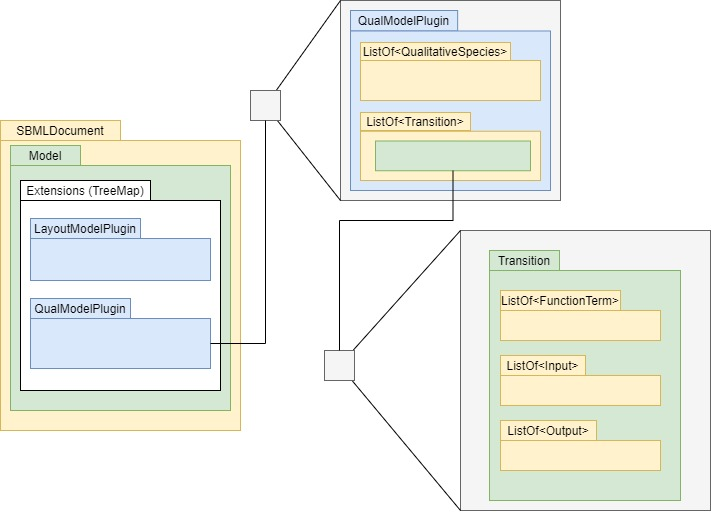
\includegraphics[scale=0.4]{Sections/Images/SBMLModel structure.jpg}
%    \caption{The SBML model reduced to its most important components}
%    \label{fig:my_label}
%\end{figure}

%Side Notes:
%Law of Demeter - Principle of least knowledge